\documentclass[french, 11pt]{article}

%-------------------------------------------------------------------------------
\usepackage[a4paper,top=1cm,bottom=2cm,left=1cm,right=1cm,marginparwidth=0.5cm]{geometry}
\usepackage{amsmath,amsfonts,amssymb,amsthm}
\usepackage[french]{babel}
\usepackage[utf8]{inputenc}
\usepackage[T1]{fontenc}
\usepackage{enumerate}
\usepackage{natbib}
\usepackage{graphicx}
\usepackage{xspace}
\usepackage{color,xcolor}
\usepackage{tikz}
\usepackage{remreset}
\usepackage{url}
\usepackage{boites}
% \usepackage{extsizes} % Permet \documentclass[french, 14pt]{extreport}
% \usepackage[a4paper,top=1cm,bottom=2cm,left=1cm,right=1cm,marginparwidth=.75cm]{geometry}
% \usepackage{minitoc}

\graphicspath{{../Figures/}}
% Environnement
\newtheorem{theorem}{Théorème}
\newtheorem{definition}{Définition}
\newtheorem{lemma}{Lemme}
\newtheorem{proposition}{Proposition}
\newtheorem*{theorem*}{Théorème}
\newtheorem*{definition*}{Définition}
\newtheorem*{proposition*}{Proposition}
\newtheorem*{corollary*}{Corollaire}
\newtheorem*{assumption*}{Hypothèse}
\newtheorem*{algorithm*}{Algorithme}
\newtheorem*{lemma*}{Lemme}
\newtheorem*{remark*}{Remarque}
\newtheorem*{exercise*}{Exercice}
\newtheorem{exercise}{Exercice}
\newcommand{\remark}{\bigskip\noindent\textbf{\textsl{Remarque.}}\xspace}
\newcommand{\remarks}{\bigskip\noindent\textbf{\textsl{Remarques.}}\xspace}
\newcommand{\parSR}[1]{\paragraph*{\textsl{#1}}\xspace}
\renewcommand{\proof}{\bigskip\noindent\underline{\textsl{Démonstration}.}\xspace}
\newcommand{\eproof}{$\blacksquare$}

% Effets, couleurs
\newcommand{\emphase}[1]{\textcolor{red}{#1}}
\newcommand{\demoProp}[1]{\noindent{\textbf{\textsl{Démonstration de la proposition \ref{#1} :}}}}
\newcommand{\itemdot}{\textbullet}

% Moments
\DeclareMathOperator{\Esp}{\mathbb{E}}
\DeclareMathOperator{\diag}{diag}
\DeclareMathOperator{\Cov}{\mathbb{C}ov}
\DeclareMathOperator{\tr}{tr}
\DeclareMathOperator{\Var}{\mathbb{V}}
\let\Pr\relax\DeclareMathOperator{\Pr}{\mathbb{P}}
\renewcommand{\d}{\text{d}}

% R, N, ...
\newcommand{\cst}{\text{cst}}
\newcommand{\Cbb}{\mathbb{C}}
\newcommand{\Ibb}{\mathbb{I}}
\newcommand{\Nbb}{\mathbb{N}}
\newcommand{\Rbb}{\mathbb{R}}
\newcommand{\Zbb}{\mathbb{Z}}

% Indicateurs

% Lois et ensembles
\newcommand{\Acal}{\mathcal{A}}
\newcommand{\Bcal}{\mathcal{B}}
\newcommand{\Ccal}{\mathcal{C}}
\newcommand{\Ecal}{\mathcal{E}}
\newcommand{\Gcal}{\mathcal{G}}
\newcommand{\Ical}{\mathcal{I}}
\newcommand{\Lcal}{\mathcal{L}}
\newcommand{\Mcal}{\mathcal{M}}
\newcommand{\Ncal}{\mathcal{N}}
\newcommand{\Pcal}{\mathcal{P}}
\newcommand{\Rcal}{\mathcal{R}}
\newcommand{\Scal}{\mathcal{S}}
\newcommand{\Ucal}{\mathcal{U}}
\newcommand{\Xcal}{\mathcal{X}}
\newcommand{\Ycal}{\mathcal{Y}}

% Comments
\newcommand{\SR}[2]{\textcolor{gray}{#1}\textcolor{red}{#2}}
\newcommand{\todo}[1]{\textcolor{red}{\`A faire~: {\sl #1}}}
\newcommand{\dessin}[1]{
\begin{center}\framebox{\begin{minipage}{\textwidth}
  \textcolor{purple}{#1}
\end{minipage}}\end{center}
\bigskip
}
\newcommand{\progres}[1]{
\begin{center}\framebox{\begin{minipage}{\textwidth}
  \textcolor{blue}{{\sl #1}}
\end{minipage}}\end{center}
\bigskip
}
\newcommand{\solution}[1]{
\begin{center}\framebox{\begin{minipage}{\textwidth}
  \noindent{\sl Solution :}
  #1
\end{minipage}}\end{center}
\bigskip
}
% \newcommand{\exemple}[1]{
% \begin{center}\framebox{\begin{minipage}{\textwidth}
%   \parSR{Exemple.}
%   #1
% \end{minipage}}\end{center}
% \bigskip
% }
\newcommand{\exemple}[1]{
\begin{breakbox}
  \parSR{Exemple.}
  #1
\end{breakbox}
\bigskip
}

\newcommand{\SRcorrect}[2]{\textcolor{gray}{#1}\textcolor{blue}{#2}}
\newcommand{\SRcomment}[1]{\textcolor{blue}{[{\sl SR: #1}]}}



% Section numbering
\usepackage{chngcntr}
\renewcommand{\thepart}{\Roman{part}}
% \counterwithout{section}{part}
\setcounter{secnumdepth}{3}
\setcounter{tocdepth}{1}

% Proposition numbering
\renewcommand{\subsubsection}{\section}
% \numberwithin{exercise}{section}
% \numberwithin{equation}{section}

% Suppression des solutions
% \renewcommand{\solution}[1]{}

\newcommand{\alglin}{/home/robin/ENSEIGN/Cours/MathBiologie/L3-ENS-Math1/Exercices/AlgLin}
\newcommand{\multivar}{/home/robin/ENSEIGN/Cours/MathBiologie/L3-ENS-Math1/Exercices/MultiVar}
\newcommand{\equadiff}{/home/robin/ENSEIGN/Cours/MathBiologie/L3-ENS-Math1/Exercices/EquaDiff}
\newcommand{\probas}{/home/robin/ENSEIGN/Cours/MathBiologie/L3-ENS-Math1/Exercices/Probas}


% %-------------------------------------------------------------------------------
% %-------------------------------------------------------------------------------
% \title{\Huge{Ce qu'un biologiste doit savoir en mathématiques}}
% \author{SR d'après \cite{Lam20} : Annexes}
% \date{\today}


\title{\normalsize{\sc École Normale Supérieure de Paris, Licence de Biologie L3}
  
  \bigskip
  \normalsize{\sc Année 2025–25}
  
  \bigskip
  \large{\bf Mathématiques I : ce qu’un biologiste ne doit pas ignorer} 
  
}
\date{Examen, le 17 janvier 2025}

%-------------------------------------------------------------------------------
%-------------------------------------------------------------------------------
\begin{document}
%-------------------------------------------------------------------------------
%-------------------------------------------------------------------------------

\maketitle

\bigskip
L'épreuve dure 2 heures. 
Les notes de cours individuelles sont autorisées.
L’usage de tout appareil électronique est interdit à l’exception d’une calculatrice.

%-------------------------------------------------------------------------------
% \section{Algèbre linéaire}
%-------------------------------------------------------------------------------
\subsubsection{\'Evolution de fréquences alléliques}
%-------------------------------------------------------------------------------

\paragraph{Dynamique de fréquences alléliques.}
Dans une population diploïde panmictique, on s’intéresse à un gène existant sous la forme de $m$ allèles. On désigne par $p_i(t)$ la proportion du pool gamétique portant l’allèle $i$  à la génération $t$ et $p(t) = (p_i(t))_{1 \leq i \leq m}$ le vecteur des fréquences alléliques à la génération $t$, qui vérifie $\sum_{1 \leq i \leq m}p_i(t) = 1$. 

On définit la matrice, supposée symétrique, $A = [a_{ij}]_{1 \leq i, j \leq p}$ où les $a_{ij}$ sont tous positifs ou nuls, mais non tous nuls. La dynamique des fréquences alléliques est donnée par
\begin{align} \label{eq:dynFreqModele}
  \forall \; i = 1 \dots m: & & 
  p_i(t+1) & = V(t)^{-1} p_i(t) \sum_{j=1}^m a_{ij} p_j(t) \\
  \text{avec} & & 
  V(t) & = \sum_{i=1}^m \sum_{j=1}^m a_{ij} p_i(t) p_j(j) = p(t)^\top \; A \; p(t), \nonumber
\end{align}
de sorte que $\sum_{1 \leq i \leq m} p_i(t+1) = 1$.

\bigskip
\begin{enumerate}
  \item Interpréter l'équation \eqref{eq:dynFreqModele}. Pourquoi $A$ est-elle supposée symétrique ? Que représente $V(t)$ ?
  \solution{$a_{ij}$ représente l'avantage relatif du génotype $(A_i, A_j)$, qui est symétrique par nature. \\
  $V(p) = p^\top A p$ est l'avantage moyen d'un descendant, du fait de la reproduction panmictique. 
  
  \remark 
  Ce modèle est paramétré à une constante près, c'est-à-dire qu'on aboutit à la même dynamique en remplaçant $A$ par $B = k A$ pour n'importe quel $k > 0$.
  }
\end{enumerate}

\paragraph{Caractérisation d'un équilibre.}
On suppose à partir de maintenant qu'il existe un équilibre $p^* = (p^*_i)_{1 \leq i \leq m}$ pour le système \eqref{eq:dynFreqModele}, c'est-à-dire vérifiant : 
$$
p(t) = p^* \qquad \Rightarrow \qquad p(t+1) = p^*,
$$
et qu'il est ``non trivial'', c'est-à-dire dans lequel tous les allèles sont présents : 
$$
\forall \; i = 1 \dots m: \qquad p^*_i > 0
$$
et on note $V^* = V(p^*) > 0$.

\begin{enumerate}
  \setcounter{enumi}{1}
  \item Montrer que, pour tout $i$ : $\sum_{1 \leq j \leq m} a_{ij} p^*_j = V^*$.
  \solution{L'équilibre $p^*$ est un point stationnaire de la dynamique \eqref{eq:dynFreqModele}, donc, en posant $p(t+1) = p(t) = p^*$, il vient
  $$
  \forall \; i = 1 \dots m: \quad V^* p^*_i = p^*_i \sum_{j=1}^m a_{ij} p^*_j,
  $$
  soit $V^* = \sum_{j=1}^m a_{ij} p^*_j, \forall i$, puisque les $p_i^*$ sont tous non nuls.. }
\end{enumerate}

\paragraph{Condition d'optimalité d'un équilibre.}
On cherche maintenant à déterminer sous quelles conditions l'équilibre (non trivial) $p^*$ correspond à un optimum pour $V$.

\begin{enumerate}
  \setcounter{enumi}{2}
  \item En écrivant tout vecteur de fréquences alléliques $p$ sous la forme $p = p^* + x$, montrer que $V^*$ est maximal ssi
  \begin{equation*} % \label{eq:dynFreqCondition}
    \forall x \in \Rbb^m \text{ tel que } \sum_{i=1}^m x_i = 0: \qquad x^\top A x \leq 0.
  \end{equation*}
  \solution{Si $p = p^* + x$, on a 
  $$
  V(p) 
  = p^\top A p
  = {p^*}^\top A p^* + 2 x^\top A p^* + x^\top A x
  = V^* + 2 x^\top A p^* + x^\top A x.
  $$
  De plus, $p$ et $p^*$ étant des vecteurs de fréquences ($1_m^\top p = 1_m^\top p^* = 1$), si $p = p^* +x$, alors $1_m^\top x = \sum_i x_i = 0$. Or on a vu que $\sum_j a_{ij} p^*_j$ est indépendant de $i$ (et égal à $V^*$), donc $A p^* = V^* 1_m$, donc
  $$
  x^\top A p^* = x^\top V^* 1_m = V^* x^\top 1_m = 0
  $$
  donc
  $$
  V(p) 
  = V^* + x^\top A x,
  $$
  $V^*$ est donc maximal, ssi $\forall p, V(p) \leq V^*$, c'est-à-dire ssi $x^\top A x \leq 0$.
  }
  %
  \item Montrer qu'on peut écrire $A$ sous la forme $A = R \Lambda R^\top$ où
  $$
  \Lambda = \text{diag}(\lambda_1, \dots, \lambda_k, 
    \lambda_{k+1}, \dots, \lambda_{k+\ell}, 
    0, \dots, 0)
  $$
  avec $k \geq 0$, $\ell \geq 0$, $k+\ell \leq m$, $\lambda_1, \dots \lambda_k > 0$ et $\lambda_{k+1}, \dots \lambda_{k+\ell} < 0$.
  \solution{
  $A$ étant symétrique, elle est diagonalisable et ses vecteurs propres sont orthogonaux. On peut donc l'écrire sous la forme $A = R \Lambda R^\top$ en mettant en premier les valeurs propres strictement positives, puis strictement négatives, puis, éventuellement, nulles. 
  }
  %
  \item Montrer l'existence de $p^*$ assure que $k \geq 1$.
  \solution{
  Si $k = 0$, alors tous les $\lambda_i$ sont négatifs (ou nuls), c'est-à-dire que $A$ est négative ($A \preceq 0$), donc
  $$
  \forall x \in \Rbb^m: \qquad 
  x^\top A x 
  = x^\top R \Lambda R^\top x 
  = y^\top \Lambda y  
  = \sum_i \lambda_i y_i^2 \leq 0 
  $$
  en posant $y = R^\top x$, or $V^* = {p^*}^\top A p^* > 0$ (car $A \geq 0$ et $p^*_i > 0$, $\forall i$), donc on a nécessairement $k \geq 1$.
  }
  \item En déduire que $V^*$ est maximal ssi $k=1$ et $\ell \geq 1$. 
  \solution{
  On a vu que, pour que $V^*$ soit maximal, il faut que $x^\top A x \leq 0$ pour tout $x$ vérifiant $\sum_i x_i = 0$, qui définit une sous-espace de dimension $m-1$. $k$ ne peut donc pas être supérieur ou égal à 2 (car alors il existerait alors au moins deux dimensions dans lesquelles $x^\top A x > 0$). \\
  La condition $\ell \geq 1$ assure seulement qu'il existe des vecteurs de fréquences $p = p^* + x$ donnant une viabilité $V(p) = V^* + x^\top A x < V^*$. 
  }
\end{enumerate}


%-------------------------------------------------------------------------------
% \section{Fonction de plusieurs variables}
% %-------------------------------------------------------------------------------
\subsubsection{Exemple de fonction de $\Rbb^2 \mapsto \Rbb$}
%-------------------------------------------------------------------------------

Soit la fonction $f: \Rbb^2 \mapsto \Rbb$ définie par
$$
f(x, y) = x^3 + y^3 - 3 xy
$$

\begin{enumerate}
  \item Déterminer les points stationnaires de la fonction $f$.
  \solution{
    Le gradient de $f$ vaut
    $$
    \nabla f = \left[\begin{array}{c} 3x^2 - 3y \\ 3y^2 - 3x \end{array}\right]
    $$
    qui est nul aux points
    $$
    a = (0, 0) \qquad \text{et} \qquad b = (1, 1).
    $$
  }
  \item Déterminer s'il s'agit de maximums, de minimums ou de points selles.
  \solution{
    La hessienne vaut
    $$
    \nabla^2 f = \left[\begin{array}{rrr} 6x & & -3 \\ -3 & & 6y \end{array}\right].
    $$
    \begin{description}
      \item[\'Etude du point $a$ :] on a 
      $$
      \nabla_a^2 f = \left[\begin{array}{rrr} 0 & & -3 \\ -3 & & 0 \end{array}\right]
      \qquad \Rightarrow \qquad 
      | \nabla_a^2 f | = -9 < 0
      $$
      donc $a$ est un point selle. Ses valeurs propres sont les racines de
      $$
      P(\lambda) = \left|\begin{array}{rrr} -\lambda & & -3 \\ -3 & & -\lambda \end{array}\right|
      = \lambda^2 - 9 
      \qquad \text{soit} \quad 
      \lambda = \pm 3.
      $$
      Tout vecteur propre associé à $\lambda = -3$ est solution de 
      $$
      \left\{\begin{array}{rcl} -3y & = & -3x \\-3x & = & -3y\end{array} \right.
      \qquad \Rightarrow \qquad 
      x = y
      \qquad \Rightarrow \qquad 
      \left[ \begin{array}{r} 1 \\ 1 \end{array} \right] \text{ est associé à $-3$}
      $$
      donc $a$ est un maximum dans la direction de la 1ère bissectrice. \\
      Tout vecteur propre associé à $\lambda = 3$ est solution de 
      $$
      \left\{\begin{array}{rcl} -3y & = & 3x \\-3x & = & 3y\end{array} \right.
      \qquad \Rightarrow \qquad 
      x = -y
      \qquad \Rightarrow \qquad 
      \left[ \begin{array}{r} -1 \\ 1 \end{array} \right] \text{ est associé à $+3$}
      $$
      donc $a$ est un minimum dans la direction de la 2ème bissectrice.
      $$
      \begin{tabular}{cc}
        direction $x = y$ & direction $x = -y$ \\
        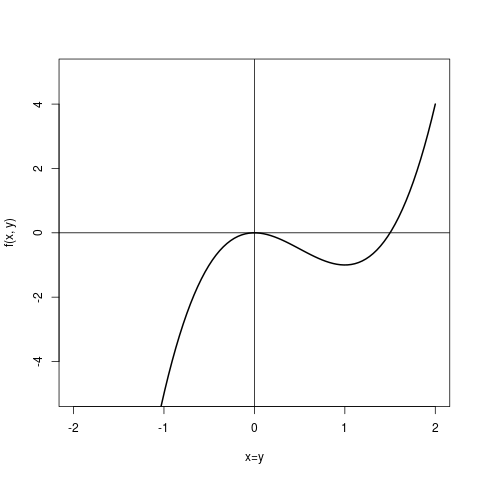
\includegraphics[width=.35\textwidth, trim=00 10 10 40, clip=]{ExempleOptimum-1ereBissectrice} &
        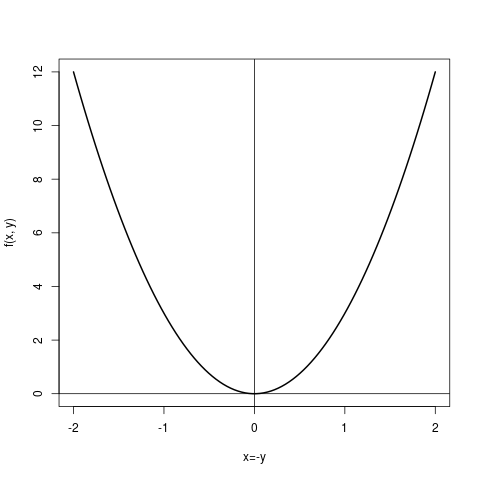
\includegraphics[width=.35\textwidth, trim=00 10 10 40, clip=]{ExempleOptimum-2emeBissectrice} \\
        $f(x, x) = 2x^3 - 3x^2$ & $f(x, -x) = 3x^2$
      \end{tabular}
      $$
      \item[\'Etude du point $b$ :] on a
      $$
      \nabla_b^2 f = \left[\begin{array}{rrr} 6 & & -3 \\ -3 & & 6 \end{array}\right]
      \qquad \Rightarrow \qquad 
      | \nabla_b^2 f | = 27 > 0, \qquad \tr(\nabla_b^2 f) = 12 > 0
      $$
      donc les deux valeurs propres de $\nabla_b^2 f$ sont positives : $b$ est donc un minimum.
    \end{description}
    Au total la surface d'équation $\{z = f(x, y)\}$ a l'aspect suivant
    $$
    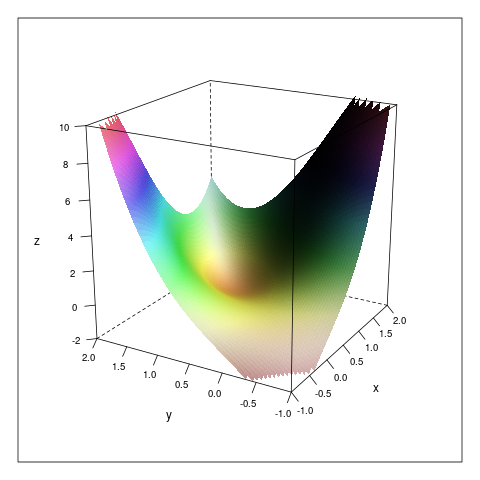
\includegraphics[width=.6\textwidth]{ExempleOptimum-surface}
    $$
  }
\end{enumerate}


%-------------------------------------------------------------------------------
% \section{Systèmes dynamiques}
\bigskip \bigskip 
%-------------------------------------------------------------------------------
\subsubsection{Système de Lorenz en 2 dimensions} 
%-------------------------------------------------------------------------------

On considère une version réduite à deux dimensions du système de Lorenz, c'est-à-dire à un couple $(x(t), y(t))_{t \geq 0}$ satisfaisant les conditions initiales
$$
x(0) = x_0, \qquad y(0) = y_0
$$
et vérifiant le système d'équations différentielles ordinaires
\begin{equation*} % \label{eq:lorenz2D}
  \left\{\begin{array}{rcl}
    \dot x & = a x - xy \\
    \dot y & = x^2 - by
  \end{array}\right.
\end{equation*}
où les coefficients $a$ et $b$ sont strictement positifs.

\paragraph{Détermination des points stationnaires et de leur stabilité.}
\begin{enumerate}
  \item Montrer que le système admet trois points stationnaires.
  \solution{
    En annulant simultanément
    $$
    F_1(x, y) = a x - xy, \qquad F_2(x, y) = x^2 - by,
    $$
    on détermine que le vecteur gradient est nul aux points 
    $$
    O = (0, 0), \qquad A = (\sqrt{ab}, a) \quad \text{et} \quad B = (-\sqrt{ab}, a).
    $$
  }
  \item Déterminer la matrice Jacobienne du système.
  \solution{
  On a
  $$
  J f = \left[\begin{array}{cc} a-y & -x \\ 2x & -b \end{array} \right].
  $$
  }
  \item En déduire la nature (stable ou instable) de chacun des points stationnaires.
  \solution{
  \begin{description}
    \item[$O = (0, 0)$ :] On a
    $$
    J_0 f = \left[\begin{array}{cc} a & 0 \\ 0 & -b \end{array} \right],
    $$
    dont les valeurs propres ($\lambda_1 = a, \lambda_2 = b)$ sont de signes opposés : $O$ est donc instable. Plus précisément, il est instable le long de l'axe des $x$ et stable le long de l'axe des $y$.
    \item[$A = (\sqrt{ab}, a)$ :] On a
    $$
    J_A f = \left[\begin{array}{cc} 0 & -\sqrt{ab} \\ 2\sqrt{ab} & -b \end{array} \right],
    $$
    donc $\tr(J_A f) = -b < 0$ et $\det(J_A f) = 2ab > 0$. Les deux valeurs propres sont donc de même signe et négatives : $A$ est donc un équilibre stable. \\
    {\sl Alternative :} Le polynôme caractéristique
    $$
    P_A(\lambda) = \lambda^2 + b \lambda + 2 ab
    $$
    a pour discriminant $\Delta = b^2 - 8 ab$. 
    \begin{itemize}
      \item Si $0 < a < b/8$, $\Delta$ est positif et les valeurs propres sont 
      $$
      \lambda_1 = \frac12 \left(-b + \sqrt{\Delta}\right) 
      \quad \text{et} \quad
      \lambda_2 = \frac12 \left(-b - \sqrt{\Delta}\right).
      $$
      comme de plus $\Delta < b^2$, les deux valeurs propres sont négatives, donc $A$ est stable.
      \item Si $a > b/8$, $\Delta$ est négatif et les valeurs propres sont 
      $$
      \lambda_1 = \frac12 \left(-b + i \sqrt{|\Delta|}\right) 
      \quad \text{et} \quad
      \lambda_2 = \frac12 \left(-b - i \sqrt{|\Delta|}\right),
      $$      
      dont la partie entière commune est $-b < 0$, donc $A$  est également stable.
    \end{itemize}
    \item[$B = (-\sqrt{ab}, a)$ :] On a alors    
    $$
    J_B f = \left[\begin{array}{cc} 0 & \sqrt{ab} \\ -2\sqrt{ab} & -b \end{array} \right]
    $$
    qui a la même trace et le même déterminant que $J_A f$ : $B$ est donc également stable. \\
    {\sl Alternative :} Le polynôme caractéristique de $J_B f$ est le même que celui de $J_A f$ donc $B$ est de même nature que $A$.
  \end{description}
  }
\end{enumerate}

\paragraph{Cas de paramètres négatifs.}
On étudie maintenant le cas où les paramètres $a$ et $b$ peuvent prendre des valeurs négatives. On ne s'attardera pas sur les cas limites $a = 0$ et/ou $b = 0$.

\bigskip
\begin{enumerate}
  \setcounter{enumi}{3}
  \item Déterminer le ou les points stationnaires et étudier sa (leur) stabilité quand $a$ est négatif ($b$ étant toujours strictement positif).
  \solution{
    Si $a < 0$ (et $b > 0$), alors $ab < 0$ donc $O$ est le seul point stationnaire, et les deux valeurs propres de $J_O f$ sont négatives, donc $O$ est stable.
  }
  \item Mener la même étude pour $a > 0$ et $b < 0$, d'une part, et pour $a < 0$ et $b < 0$, d'autre part.
  \solution{
  \begin{description}
    \item[$a > 0, b < 0$ :] Alors $ab < 0$ donc $O$ est le seul point stationnaire, mais les deux valeurs propres de $J_O f$ sont positives, donc $O$ est instable. 
    \item[$a < 0, b < 0$ :] Alors $ab > 0$ donc $O$, $A$ et $B$ sont stationnaires.
    \begin{itemize}
      \item Le valeurs propres de $J_O f$ sont alors de signes opposés, donc $O$ est instable.
      \item On a $\tr(J_A f) = \tr(J_B f) = -b > 0$ et $\det(J_A f) = \det(J_B f) = 2 ab > 0$. Les deux valeurs propres sont donc positives et $A$ et $B$ sont donc instables. \\
      {\sl Alternative:} Le discriminant de $P_A(\lambda)$ (et donc de $P_B(\lambda)$) vaut alors $\Delta = b^2 - 8ab > b^2 > 0$. Les deux valeurs propres
      $$
      \lambda_1 = \frac12 \left(-b + \sqrt{\Delta}\right) 
      \quad \text{et} \quad
      \lambda_2 = \frac12 \left(-b - \sqrt{\Delta}\right).
      $$
      sont alors de signe opposé : $A$ et $B$ sont donc instables.
    \end{itemize}
  \end{description}
  }
\end{enumerate}



%-------------------------------------------------------------------------------
% \section{Probabilités}
\bigskip \bigskip 
%-------------------------------------------------------------------------------
\subsubsection{Processus de Galton-Watson avec survie des descendants}
%-------------------------------------------------------------------------------

\paragraph{Nombre et survie des descendants.}
Dans une population asexuée, un individu a au cours de sa vie $N$ enfants, où $N$ suit une loi de Poisson de paramètre $\theta$. On suppose de plus que chacun des $N$ enfants survit à la naissance avec probabilité $p$, indépendamment des autres et de $N$. On note $\varepsilon_i$ la variable qui vaut 1 si le $i$-ème enfant survit et 0 sinon. On note $K$ le nombre d'enfants survivants.

\begin{enumerate}
  \item Donner la fonction génératrice $f$ de $N$.
  \solution{
    C'est la fonction génératrice d'une loi de Poisson de paramètre $\theta$:
    $f(s) = \Esp(s^N) = \exp(\theta(s-1))$.
  }
  %
  \item Rappeler la fonction génératrice $g$ de $\varepsilon_1$.
  \solution{
    C'est la fonction génératrice d'une loi de Bernoulli de paramètre $p$:
    $g(s) = \Esp(s^{\varepsilon_1}) = 1 - p + ps$.
  }
  %
  \item \'Ecrire $K$ à partir de $N$ et des $\varepsilon_i$.
  \solution{
    $K$ est la somme des indicatrices de survie $\varepsilon_i$ des $N$ enfants, soit
    $K = \sum_{i=1}^N \varepsilon_i$.
  }
  %
  \item En déduire la fonction génératrice $h$ de $K$, puis la loi de $K$.
  \solution{
    D'après les propriétés des fonctions génératrices, on a 
    $$
    h(s) = f \circ g(s) = \exp[\theta(1 - p + ps -1)] = \exp[p \, \theta(s -1)]
    $$
    $K$ suit donc une loi de Poisson de paramètre $p \, \theta$: $K \sim \Pcal(p \, \theta)$.
  }
  %
\end{enumerate}

\paragraph{Devenir de la population.}
On considère, d'une part, un processus de Bienaymé-Galton-Watson $(Y_n)_{n\geq 0}$ où chaque individu laisse à la génération suivante un nombre d'enfants de même loi que $N$ et, d'autre part, un processus de Bienaymé-Galton-Watson $(Z_n)_{n\geq 0}$ où chaque individu laisse à la génération suivante un nombre d'enfants de même loi que $K$. On suppose que $Z_0=1$ et on note $q$ la probabilité d'extinction du processus $(Z_n)_{n\geq 0}$.
\bigskip
\begin{enumerate}
  \setcounter{enumi}{4}
  \item Donner une équation de point fixe caractérisant $q$ et donner une condition sur $\theta$ et $p$ pour que $q$ soit strictement inférieure à 1.
  \solution{
    D'après les propriétés des processus de Galton-Watson, on sait que $q$ est la plus petite racine de l'équation 
    $$
    q = h(q)
    $$
    et que la probabilité d'extinction est strictement inférieure à 1 si l'espérance de $K$ est strictement supérieure à 1, soit, puisque $K \sim \Pcal(p \, \theta)$, 
    $$
    p \, \theta > 1.
    $$
  }
  %
  \item  Comment construire la généalogie du processus $Z$ à partir de celle du processus $Y$ ?
  \solution{
    Partant de la généalogie du processus $Y$, il suffit de ``tuer'' chaque individu (et toute sa descendance) avec probabilité $1 - p$.
% Correction AL: La totalité des points s'ils disent qu'il faut "supprimer chaque noeud avec proba $1-p$", du bonus s'ils disent "indépendamment" et encore plus de bonus s'ils disent "chaque noeud et toute sa descendance"
  }
  %
\end{enumerate}


%-------------------------------------------------------------------------------
%-------------------------------------------------------------------------------
\end{document}
%-------------------------------------------------------------------------------
%-------------------------------------------------------------------------------


